\documentclass[titlepage, 12pt]{article}

\usepackage[margin=1in]{geometry}
\usepackage[hidelinks]{hyperref}
\usepackage{amsmath}
\usepackage{float}
\usepackage{graphicx}
% \usepackage{newtxtext}  % WHY IS THIS HERE
\usepackage{listings}
\usepackage{color}

% Default fixed font does not support bold face
\DeclareFixedFont{\ttb}{T1}{txtt}{bx}{n}{10} % for bold
\DeclareFixedFont{\ttm}{T1}{txtt}{m}{n}{10}

% Define colors
\definecolor{deepblue}{rgb}{0,0,0.5}
\definecolor{deepred}{rgb}{0.6,0,0}
\definecolor{deepgreen}{rgb}{0,0.5,0}


% Python style for highlighting
\newcommand\pythonstyle{\lstset{
    language=Python,
    basicstyle=\ttm,
    otherkeywords={self},             % Add keywords here
    keywordstyle=\ttb\color{deepblue},
    emph={bin,_prod,__name__},          % Custom highlighting
    emphstyle=\ttb\color{deepred},    % Custom highlighting style
    stringstyle=\color{deepgreen},
    commentstyle=\color{deepgreen},
    frame=tb,
    % Any extra options here
    showstringspaces=false
}}
\newcommand\pythonexternal[2][]{{\pythonstyle\lstinputlisting[#1]{#2}}}


% Author information
\title{ENCM 467 Lab 2\\Static and Dynamic Behaviour of MOSFET inverters}
\author{Andreas Smit}
\date{September 28, 2020}

% Settings
\setlength{\parindent}{0pt}

\begin{document}
    \maketitle

    \section{Static Inverter Measurements}
    \subsection{Static Linearly Loaded Inverter}
    In LT spice the Linearly loaded inverter is built as shown below,
    \begin{figure}[H]
        \centering

        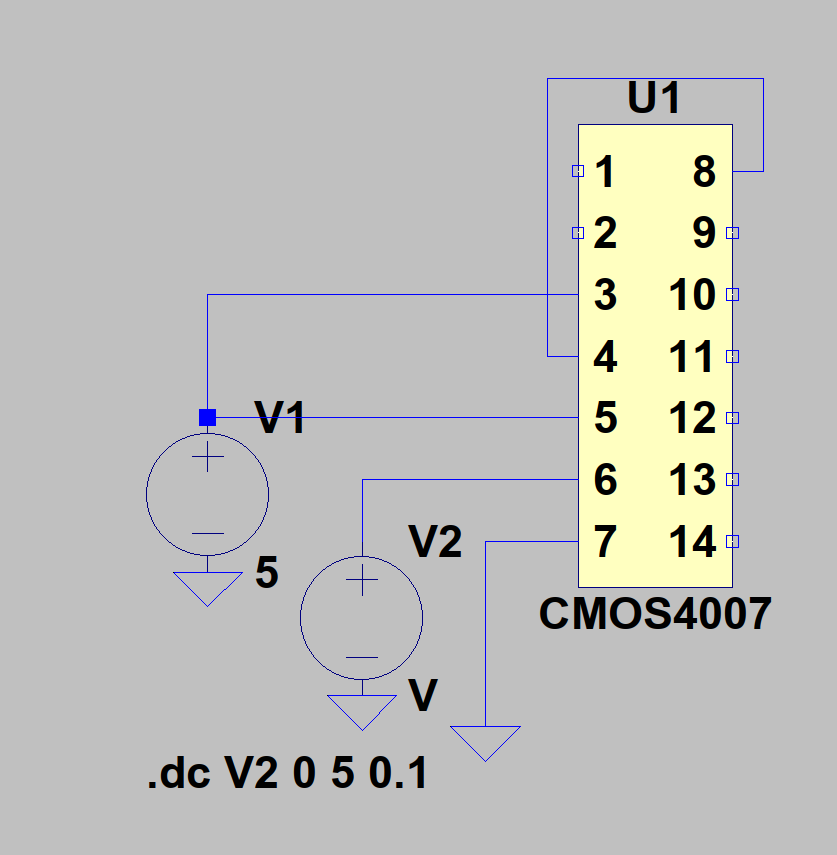
\includegraphics[width=0.6\textwidth]{figures/part_2a_sat_circ.png}
        \caption{The Linearly Loaded inverter in LT Spice with the
        load NMOS in Saturation}
        \label{fig:2a_sat_circ}
    \end{figure}
    The following is the voltage transfer characteristic is obtained for
    the circuit in figure \ref{fig:2a_sat_circ}.
    \begin{figure}[H]
        \centering
        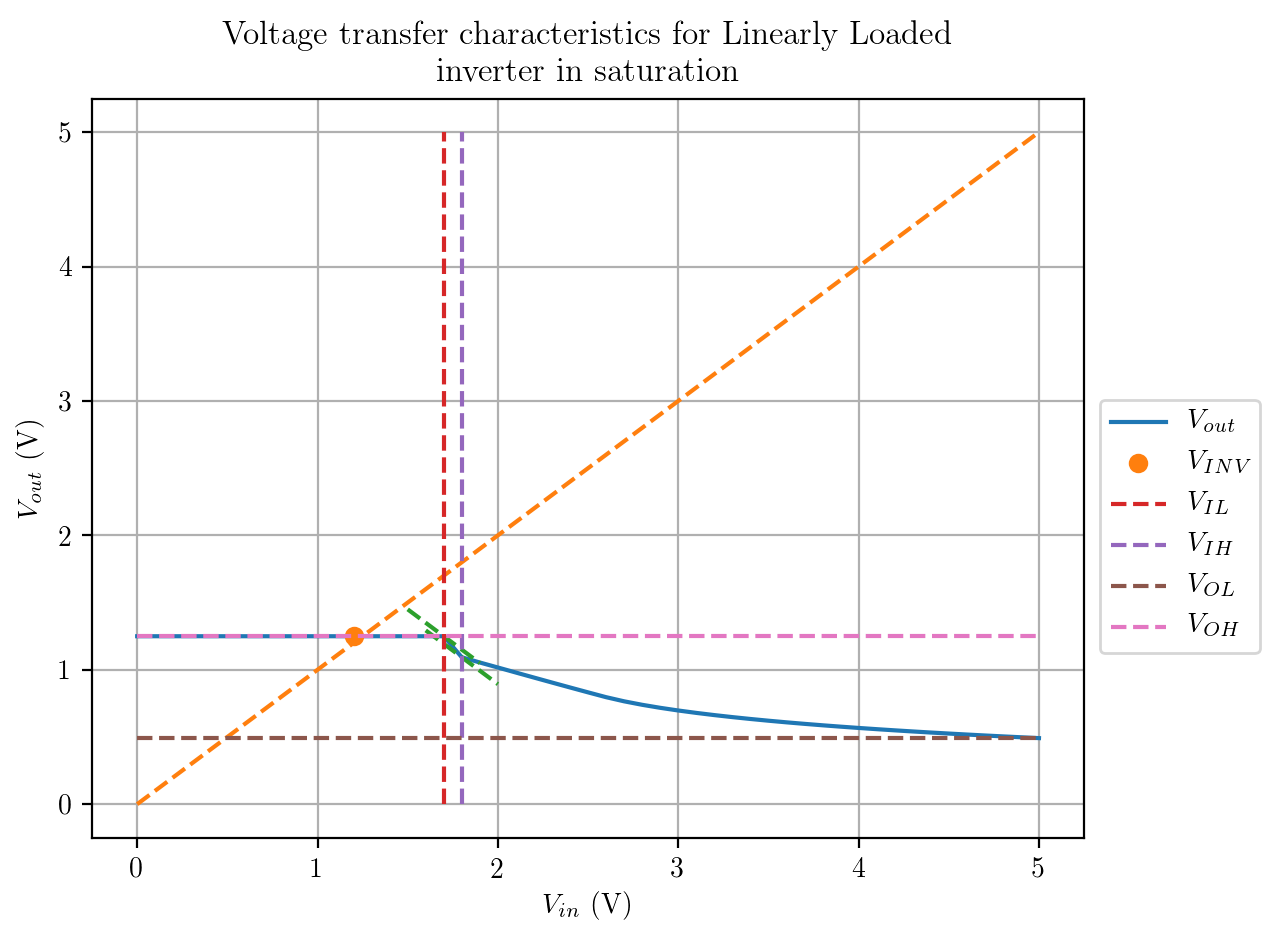
\includegraphics[width=0.6\textwidth]{figures/part_2a_sat.png}
        \caption{The voltage transfer characteristics for the linearly
            loaded inverter from figure \ref{fig:2a_sat_circ}.}
            \label{fig:2a_sat}
    \end{figure}
    The critical points in figure \ref{fig:2a_sat} are calculated using
    the python script in appendix \ref{sec:python} and are given in the
    table in appendix \ref{sec:data_tab}. The python script using the
    following formulas to calculate the data in the table in appendix
    \ref{sec:data_tab}.
    \begin{align}
        \frac{dV_{out}}{dV_{in}}\bigg|_{V_{in}=V_{IL}} &= -1\\
        \frac{dV_{out}}{dV_{in}}\bigg|_{V_{in}=V_{IH}} &= -1\\
        V_{out}\bigg|_{V_{in}= 0V} &= V_{OH}\\
        V_{out}\bigg|_{V_{in}= 5V} &= V_{OL}\\
        V_{out}\bigg|_{V_{in} = V_{INV}} &= V_{in}\\
        G &= \frac{V_{OL} - V_{OH}}{V_{IH} - V_{IL}}\\
        NM_L &= V_{IL} - V_{OL}\\
        NM_H &= V_{OH} - V_{IH}
    \end{align}

    Next the linearly loaded inverter is modified to have the load nMOS
    in triode. As the body is grounded, $V_{B} \neq V_{S}$ so the body
    effect must be considered. This raises the threshold voltage for the
    nMOS so we must raise the gate voltage higher to place the nMOS into
    triode. I chose to raise the gate voltage to 10V which should be
    high enough to place the nMOS device in triode. The modified circuit
    is shown below.
    \begin{figure}[H]
        \centering

        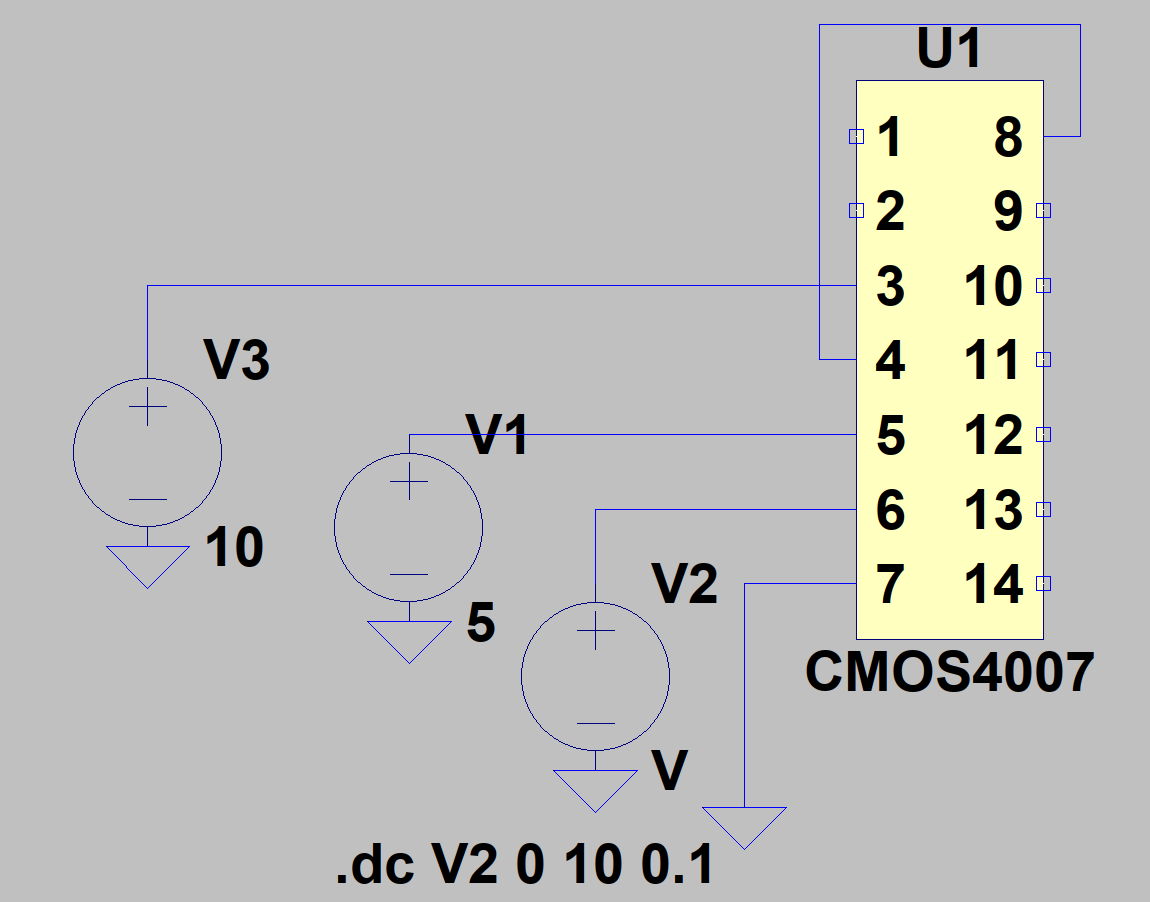
\includegraphics[width=0.6\textwidth]{figures/part_2a_tri_circ.png}
        \caption{The linearly loaded inverter in LT spice with the load
        nMOS in triode.}
    \end{figure}
    The voltage transfer plot is then given below.
    \begin{figure}[H]
        \centering
        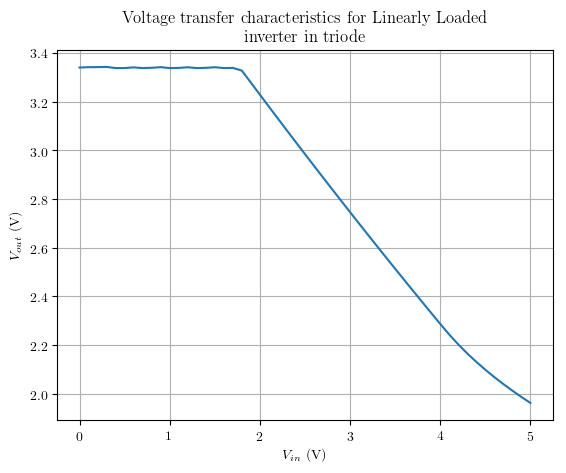
\includegraphics[width=0.6\textwidth]{figures/part_2a_tri.png}
        \caption{The voltage transfer characteristics for the linearly
        loaded inverter in triode.}
    \end{figure}
    The critical values are calculated again using the python script in
    Appendix \ref{sec:python}. However as the slope of the VTC is always
    greater than -1, the definitions of $V_{IL}$ and $V_{IH}$ can't be
    met, so 0V and 5V will be used respectively for calculating noise
    margins and gain.

    \subsection{Static CMOS Inverter}
    The CMOS inverter is built in LT spice as shown below.
    \begin{figure}[H]
        \centering
        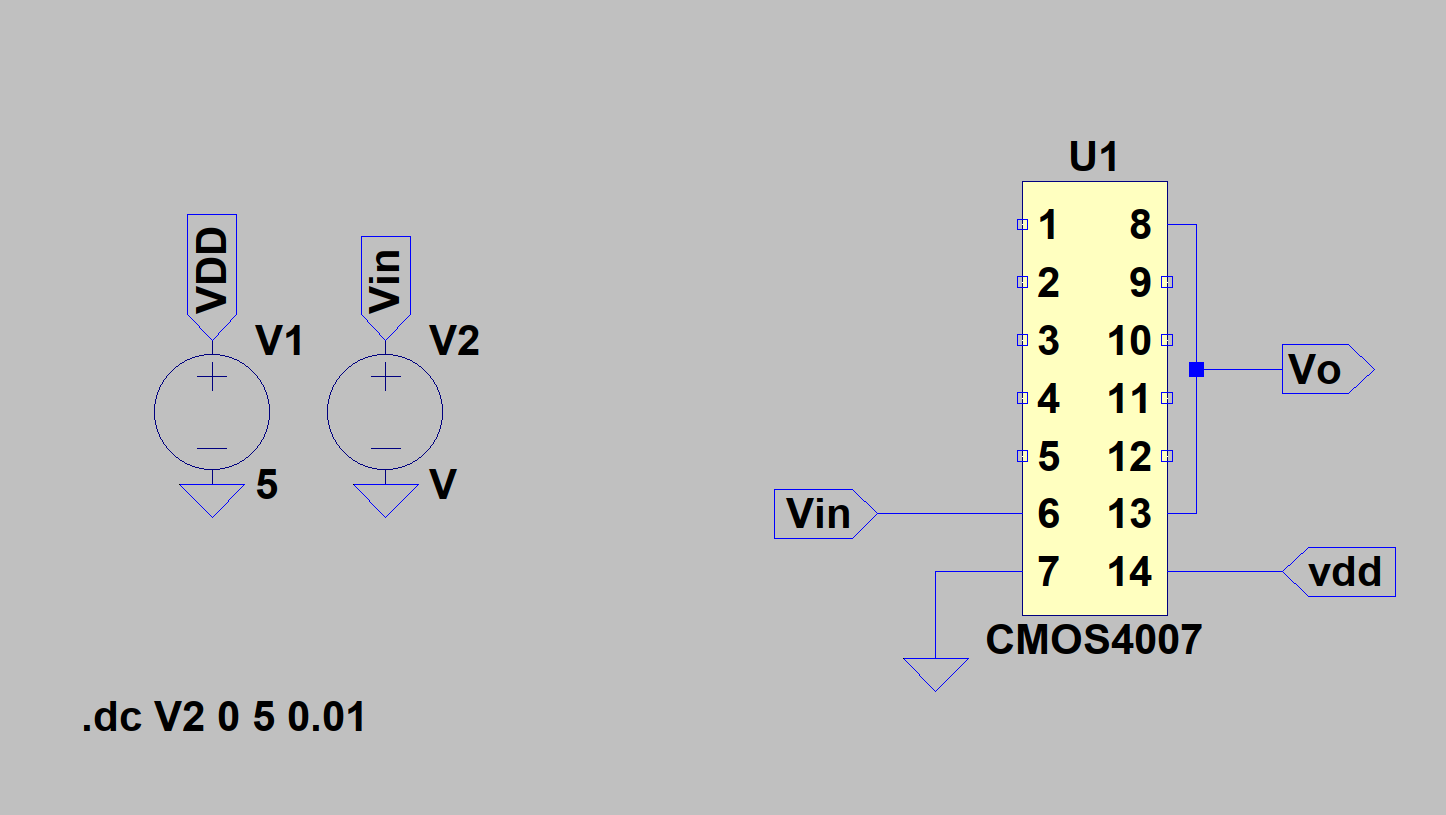
\includegraphics[width=0.6\textwidth]{figures/part_2b_circ.png}
        \caption{The CMOS inverter in LT Spice}
        \label{fig:2b_circ}
    \end{figure}
    The voltage transfer curve of the circuit in figure
    \ref{fig:2b_circ} is shown below.
    \begin{figure}[H]
        \centering
        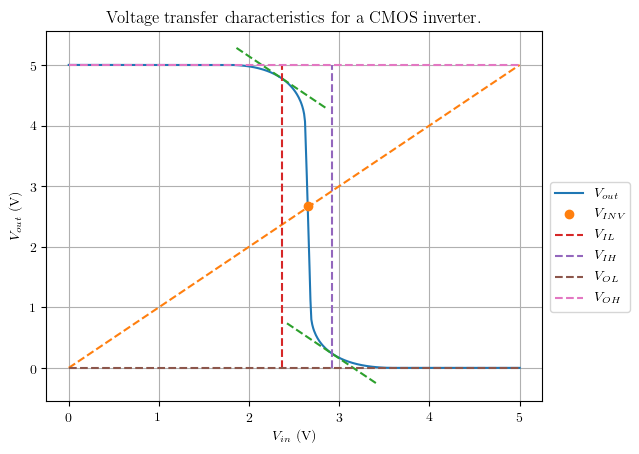
\includegraphics[width=0.6\textwidth]{figures/part_2b.png}
        \caption{The voltage transfer characteristic of the CMOS
        inverter from figure \ref{fig:2b_circ}.}
    \end{figure}
    The critical CMOS values are calculated using the python script from
    appendix \ref{sec:python} and are given in the table in appendix
    \ref{sec:data_tab}.

    \subsection{Analysis of Static Inverter Behaviour}
    First we will look at the linearly loaded inverter in saturation.
    Its two major advantages are a high low noise margin ($NM_L =
    1.21V$) and a gain comparable to the CMOS ($G=-7.5$). However its
    disadvantages far out way its advantages. It drains power when in a
    static position of logic 1 or 0, has a negative high noise margin
    ($NM_H = -0.560V$), and its logic levels are very bad for a 5V
    logic system.

    Next we will look at the linearly loaded inverter in with the load
    in triode. Its two major advantages over the previous design are a
    higher max output voltage and the inverter threshold voltage lies
    is more centered between the min and max output voltages. However
    again its disadvantages far out way the advantages. This setup
    requires an external power supply for the gate voltage, and has
    negative noise margins for both the high and low logic levels.

    Finally we will look at the CMOS inverter. The CMOS inverters
    advantages are clear. It has large noise margins for both the high
    and low logic levels, has rail to rail operation, doesn't drain
    power when at a static voltage level (besides from leakage
    currents), and has a high gain. The disadvantages of the CMOS are
    much fewer, but it is more expensive to produce and will take more
    chip area then the saturated linearly loaded inverter as the pMOS
    needs a larger area.

    Neither the saturated or triode linearly loaded inverter are useful
    as a gate in a digital system. Both designs have negative noise
    margins making them incredibly prone to logic errors without an
    additional converter to fix the logic levels.

    \section{Dynamic Inverter Measurements}
    \subsection{Dynamic Resistively Loaded Inverter Measurements}
    The resistively loaded inverter built in LT spice shown below is put
    through a transient response.
    \begin{figure}[H]
        \centering
        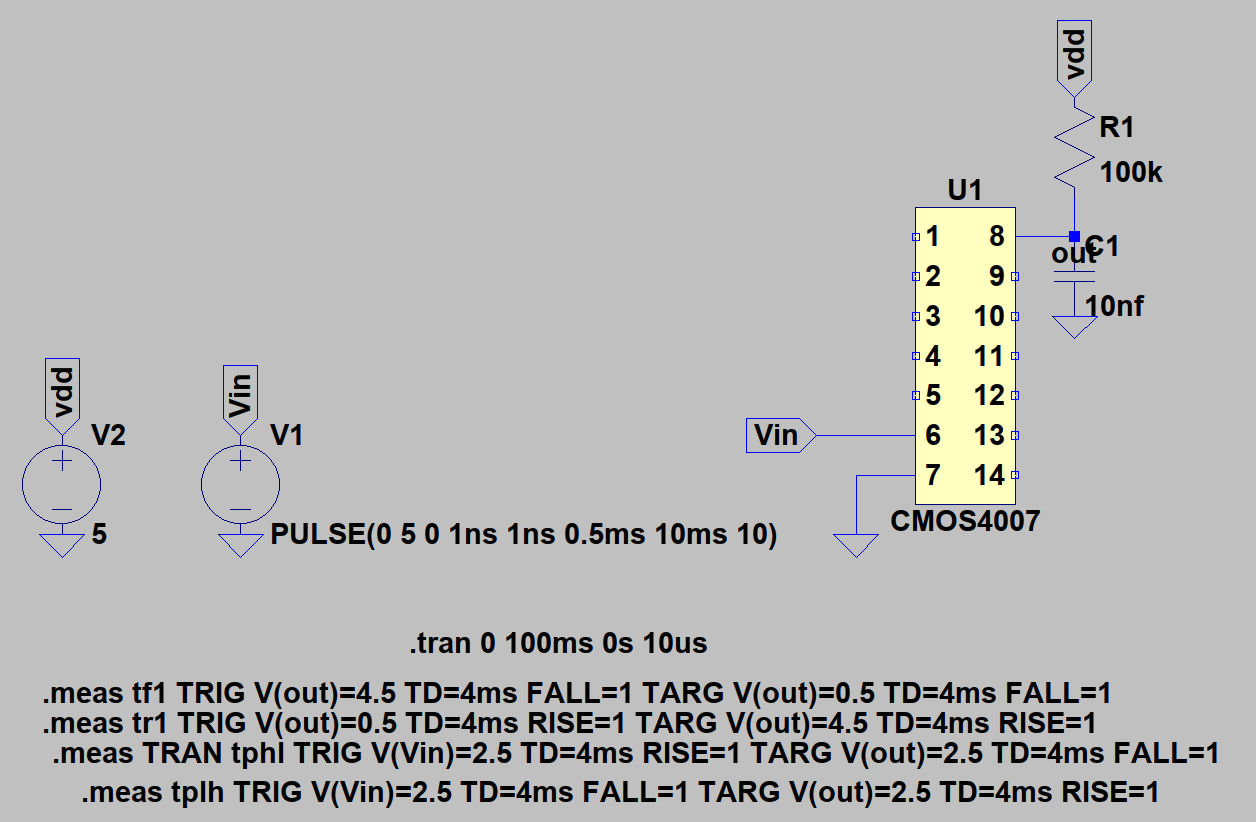
\includegraphics[width=0.6\textwidth]{figures/part_3a_circ.png}
        \caption{The resistively loaded inverter built in LT Spice}
    \end{figure}
    The transient response is shown below.
    \begin{figure}[H]
        \centering
        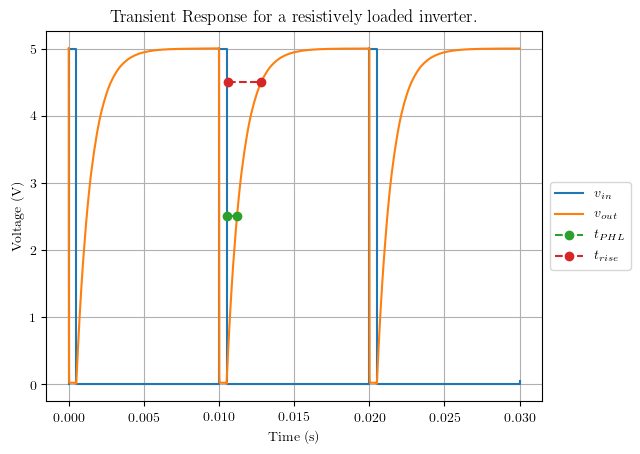
\includegraphics[width=0.6\textwidth]{figures/part_3a.png}
        \caption{The transient response of the resistively loaded
            inverter. Note that as $t_{fall}$ and $t_{PHL}$ are both
            very small compared to $t_{rise}$ and $t_{PLH}$ they aren't
        shown on the graph.}
    \end{figure}
    The critical times are calculated using the measure statements in
    the LT spice circuit. $t_{rise}$ is the time it takes for the
    output voltage to rise from 10\% $V_{DD}$ to 90\% $V_{DD}$.
    Similarly $t_{fall}$ is teh time it takes for the output voltage to
    fall from 90\% $V_{DD}$ to 10\% $V_{DD}$. $t_{PHL}$ and $t_{PLH}$
    are the times it takes for the voltage to reach $\frac{1}{2}V_{DD}$
    when the output is falling and rising respectively. $t_s$ is the
    average of $t_{PHL}$ and $t_{PLH}$. The rise and fall times are so
    drastically different do to the charging and discharging of the
    capacitor through different paths. When $V_{in}$ goes high the
    nMOS enters triode. This causes it to act as a resistor with
    resistance in the $k\Omega$. The charged capacitor then discharges
    through the nMOS to ground. When $V_{in}$ goes low, the nMOS becomes
    cut off so the capacitor will start charging through the 100k
    resistor. Because the 100k resistor is about 2 orders of magnitude
    greater in resistance then the nMOS in triode, it takes about 100
    times as long for the voltage to rise as opposed to fall.

    \subsection{Dynamic CMOS measurements}
    The CMOS inverter built in LT spice shown below is put through a
    transient response.
    \begin{figure}[H]
        \centering
        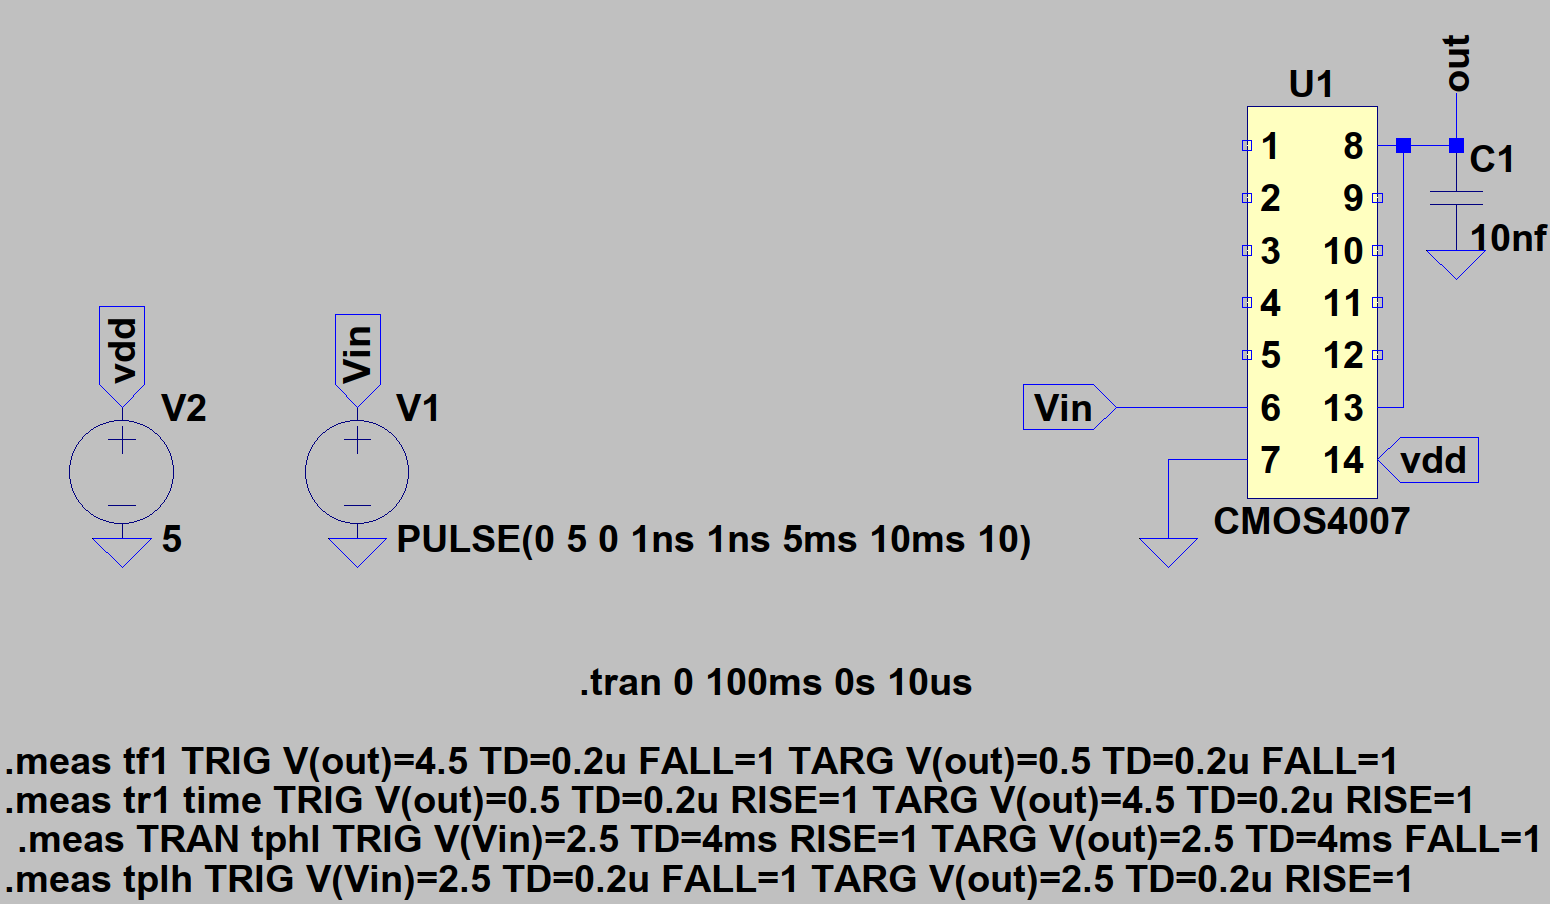
\includegraphics[width=0.6\textwidth]{figures/part_3b_circ.png}
        \caption{The CMOS inverter circuit with transient analysis}
    \end{figure}
    The transient response is then shown below,
    \begin{figure}[H]
        \centering
        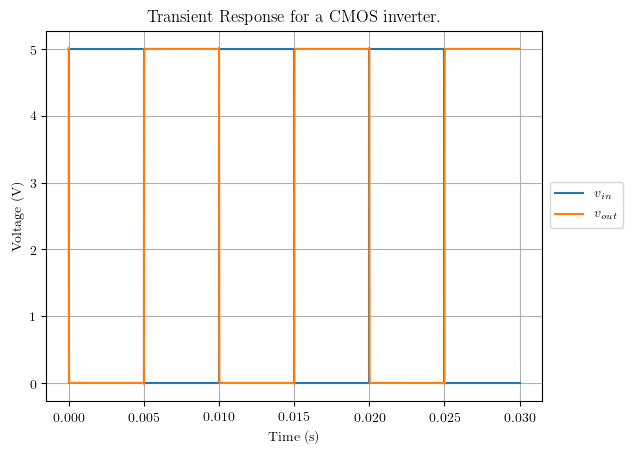
\includegraphics[width=0.6\textwidth]{figures/part_3b.png}
        \caption{The transient response of the CMOS inverter. Note that
            as the timings are very small compared to the 100Hz clock
        they aren't shown on the graph.}
    \end{figure}
    The timing values are again calculated using the measure statements
    in LT spice and are shown in the table in appendix
    \ref{sec:data_tab}.

    \subsection{Analysis of Dynamic response}
    While the CMOS and resistively loaded inverter have similar fall
    times, the rise time of the resistively loaded inverter is
    significantly higher then the CMOS inverter. This makes the CMOS
    inverter preferable for higher speed applications as it can be
    switched on and off much faster then the resistively loaded inverter
    without logic errors occurring.

    Both the CMOS and resistively loaded inverters are effected by the
    internal capacitances of the MOSFETs used to make them and load
    capacitance in determining the total propagation delay. However as
    discussed above the load resistor in the resistively loaded inverter
    greatly adds to the rise time.


    \appendix
    \pagebreak
    \section*{Appendices}
    \section{Python Code for Data Analysis}\label{sec:python}
    \pythonexternal{lab2.py}
    \section{Data Tables}\label{sec:data_tab}
    \begin{table}[H]
        \centering
        \caption{Static Values for the Inverter Voltage Transfer
        Characteristics}
        \begin{tabular}{c|c|c|c}
            & Linearly Loaded & Linearly Loaded & CMOS\\
            & Saturation & Triode & \\
            \hline
            $V_{IL}$ & 1.7 & N/A (0) & 2.35\\
            $V_{IH}$ & 1.8 & N/A (5) & 2.92\\
            $V_{OH}$ & 1.25 & 3.40 & 5\\
            $V_{OL}$ & 0.49 & 1.96 & 0\\
            $V_{INV}$ & 1.25 & 2.84 & 2.67\\
            Gain at $V_{INV}$ & -7.5 & -0.288 & -8.77\\
            $NM_L$ & 1.21 & -1.96 & 2.35\\
            $NM_H$ & -0.560 & -1.6 & 2.08\\
        \end{tabular}
    \end{table}

    \begin{table}[H]
        \centering
        \caption{Dynamic values measured for the resistively loaded inverter
        and the CMOS inverter.}
        \begin{tabular}{c|c|c}
            & Resistively Loaded Inverter & CMOS inverter\\
            \hline
            $t_{rise}$ & 2.20 ms & 11.72 $\mu$s\\
            $t_{fall}$ & 11.69 $\mu$s & 11.66 $\mu$s\\
            $t_{PHL}$ & 5.39 $\mu$s & 5.42 $\mu$s\\
            $t_{PLH}$ & 0.695 ms & 4.77 $\mu$s\\
            $t_s$ & 350 $\mu$s & 5.10 $\mu$s
        \end{tabular}
    \end{table}
\end{document}
